\cfoot{\page\textbackslash \totalp} %Skal vise x antal sider af y
\chapter{PICTURE}
Lorem ipsum dolor sit amet, consectetur adipiscing elit. Integer finibus laoreet sapien eu imperdiet. Duis diam turpis, aliquam at odio in, facilisis finibus massa. Suspendisse vel nibh iaculis, sodales nulla at, auctor neque. Vivamus quis enim sagittis, vehicula ligula in, ullamcorper arcu. Quisque eleifend vulputate urna, sit amet maximus dui ornare in. Integer id urna ipsum. Suspendisse facilisis nulla quis nisi convallis pellentesque vel at lorem. Mauris non venenatis quam, at interdum felis.

Phasellus ornare ligula ac viverra consectetur. Nam hendrerit, tellus sit amet molestie scelerisque, ipsum urna hendrerit orci, eu tincidunt ante leo at nibh. Aenean molestie cursus purus, eu euismod neque tristique nec. Praesent lacus magna, dapibus id tellus ut, volutpat molestie ex. Duis varius sem et nulla lobortis, id auctor libero blandit. Donec tristique suscipit risus sagittis tincidunt. In vel ornare purus. Morbi gravida eleifend semper. Mauris et lacus finibus, dignissim urna nec, eleifend nulla. Phasellus ac tortor quis orci ultricies congue sed eget diam.

\begin{center}
\begin{figure}
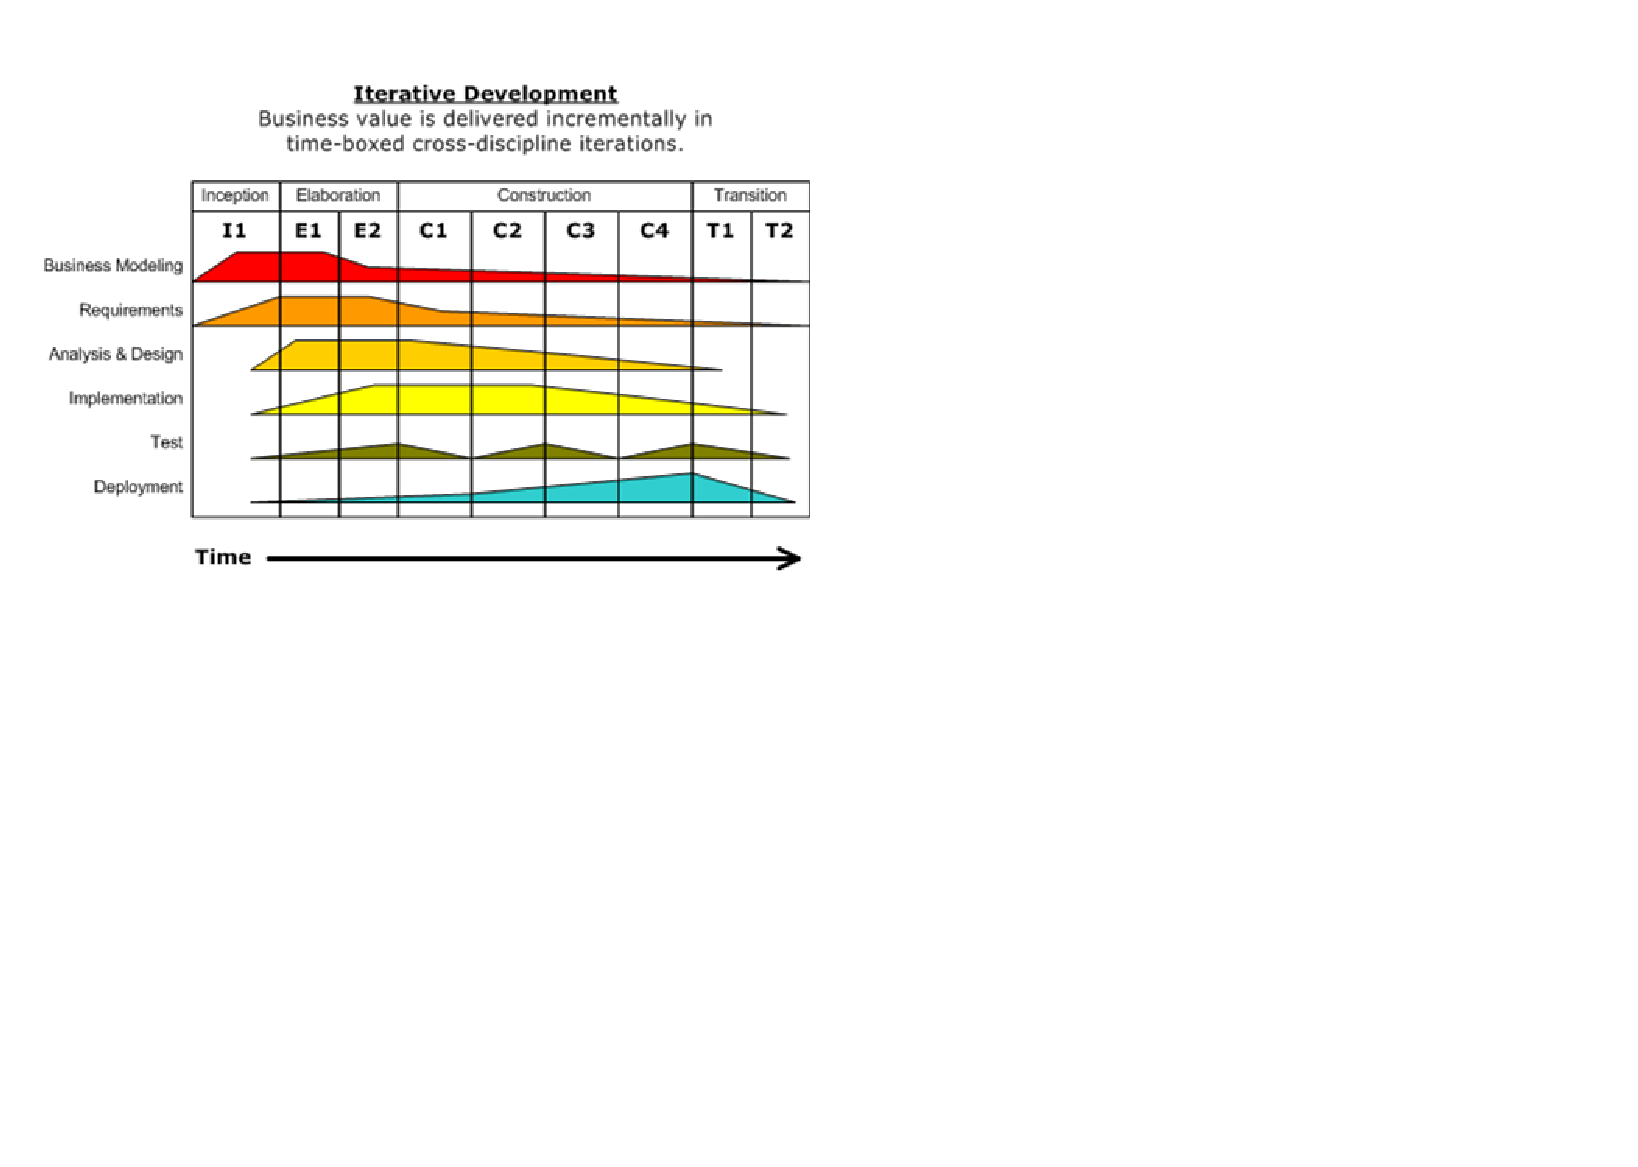
\includegraphics[trim = 0mm 100mm 100mm 500mm]{./UPmetode.eps}
\caption{Iterativ udvikling}
\end{figure}
\end{center}